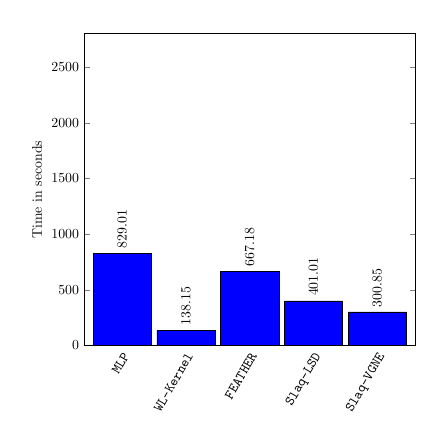
\begin{tikzpicture}[scale=0.5, every node/.style={scale=1.0}]
    \begin{axis}[
        width  = 0.825*\textwidth,
        height = 9.5cm,
        ymin=0,ymax=2800,
        ytick={0,500,1000,1500,2000,2500},
        major x tick style = transparent,
        ybar=5*\pgflinewidth,
        bar width=42.0pt,
%        ymajorgrids = true,
%        xlabel = {Model},
        ylabel = {Time in seconds},
        symbolic x coords={
MLP,
WL-Kernel,
FEATHER,
Slaq-LSD,
Slaq-VGNE
},
        xtick=data,
	y tick label style={
%		rotate=90,
    		/pgf/number format/.cd,
   		fixed,
   		fixed zerofill,
    		precision=0,
		1000 sep={}},
%	yticklabel pos=right,
%        xtick = data,
        x tick label style={
        		rotate=60,
		font=\tt,
		anchor=north east,
		inner sep=0mm
		},
%		font=\small},
%        scaled y ticks = false,
	%%%%% numbers on bars and rotated
        nodes near coords,
        every node near coord/.append style={rotate=90, 
        								   anchor=west,
%								   font=\footnotesize,
								   /pgf/number format/.cd,
								   	fixed zerofill,
									precision=2
								   },
        %%%%%
%        enlarge x limits=0.03,
        enlarge x limits=0.15,
%        enlarge x limits=0.25,
        legend cell align=left,
        legend pos=south east,
%        legend style={
%                at={(1,1.05)},
%                anchor=south east,
%	        nodes={rotate=90},%%%%% rotate text in legend
%                at={(0.125,0)},
%                at={(0.125,0)},
%                at={(0.8775,0)},
%                at={(0.89,0.02)},
%                anchor=south,
%                column sep=1ex
%        },
%        axis x line*=bottom
    ]
\addplot[fill=blue,opacity=1.00]
coordinates {
(MLP,829.01)
(WL-Kernel,138.15)
(FEATHER,667.18)
(Slaq-LSD,401.01)
(Slaq-VGNE,300.85)
};
\end{axis}
\end{tikzpicture}
